\section{\texorpdfstring{\ouralgoss}: Localizing in Presence of Authorized Users}
\label{sec:auth}
\label{sec:mtlss}

We have implicitly assumed till now that the only transmitters present
in the area are the intruders which need to be localized.  In this
section, we adapt our \ouralgo approach described in the previous
section to the setting wherein there may be authorized transmitters in
the background and the localization technique must take their presence
into account. In particular, in a shared spectrum paradigm, there are
primary users and an evolving set of active secondary users
transmitting in the background. The key challenge comes from the fact
that the set of authorized users is not static and changes over time
as allocation requests are granted and/or active secondary users
become inactive over time.

One simple way to handle background users is to just localize every
transmitter, and then remove the authorized users. However, any
localization approach (including ours) is susceptible to performance
degradation with increase in number of transmitters to be localized,
especially if some of them are situated close together. Thus, this
simple approach of localizing every transmitter is unlikely to be
effective, as shown in our evaluations, especially when the number of
primaries and active secondaries can be large. Thus, here, we develop
an approach based on learning PDs in real-time in response to changes
in the set of secondary users.

\begin{figure}
	\centering
	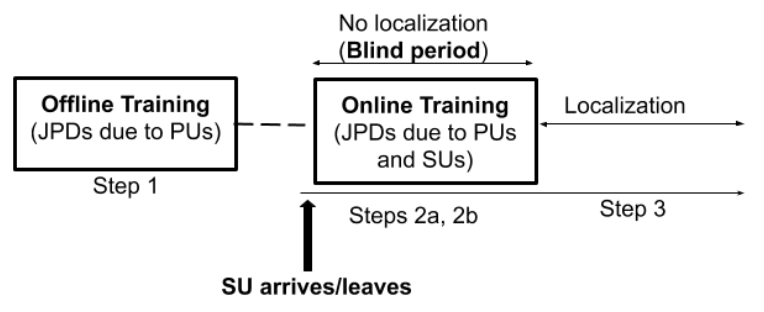
\includegraphics[width=0.7\textwidth]{chapters/ipsn/figures/map**2.png}
	\caption{\ouralgoss's overall approach}
	\label{fig:auth}
\end{figure}

\softpara{\ouralgoss: Localizing with Authorized Users}. Our problem
is to localize intruders in a shared spectrum system with fixed
primaries and changing set of secondaries.  Our \ouralgoss approach
uses a combination of a priori (offline) and online training to
construct JPDs for appropriate hypotheses based on gathered
observations, and then use these JPDs to localize intruders in
real-time using the \ouralgo approach described in the previous
section. We start with defining a few useful notations.

We use \Pa to denote the set of (fixed) primaries, and \Ka to denote
the set of secondaries at a given instant, and \ii to denote the \jth
configuration of intruders (we can assume the zero-th configuration to
represent no intruders). We use $\tau = \Pa \cup \Ka \cup \ii$ to denote the
set to all transmitters (authorized and unauthorized) at a given
instant.  Finally, we use $\pd(\vx | (\tau = X))$ to denote the joint
probability distribution (JPD) of observation vectors from the
deployed sensors when the prevailing hypothesis is that the set $\tau$
of transmitters is $X$. \ouralgoss is the sequence of following steps.
\begin{packedenumerate}
	\item
	(Offline Step.) Construct JPDs $\pd(\vx | \Pa)$ and $\pd(\vx | \tau = (\ii \cup \Pa))$ for all $j$. Since these JPDs 
	are independent of the secondaries, they do not change and
	can be done once a priori.
	\item
	(Online Steps.) Whenever \Ka (set of secondaries) changes:
	\begin{packedalpha}
		\item Construct JPD $\pd(\vx | \tau = (\Pa \cup \Ka))$. 
		\item Compute $\pd(\vx | \tau = (\Pa \cup \ii \cup
                  \Ka))$ for all $j$, from above constructed JPDs,
                  viz., $\pd(\vx | \Pa)$, $\pd(\vx | \tau = (\ii \cup
                  \Pa))$, and $\pd(\vx | \tau = (\Pa \cup \Ka))$. See
                  the below observation.
	\end{packedalpha}
	\item
	(Real-time Localization.) Periodically, each sensor sends its
          observation to a centralized entity (spectrum
          manager) which uses \ouralgo to localize any intruders
          present. Here, localization essentially means determining
          the most likely prevailing hypothesis among the hypotheses
          $\tau = (\Pa \cup \ii \cup \Ka)$, based on the JPDs $\pd(\vx | \tau = (\Pa \cup \ii \cup \Ka))$ constructed in earlier
          steps.
\end{packedenumerate}

Note that steps 1 and 2a are essentially learning the authorized users' signal charecteristics and view them as the "background signals". 
If there are no authorized users, then the background signals are "quite". Else, then the background signals have some "sound".
We now state the observation that forms the basis of JPD computation
in Steps 2b; note that the noise due to sensor's hardware gets
duplicated when ``adding'' two JPDs, but can be easily removed.
\begin{obs}
  The JPD $\pd(\vx | (\tau = A \cup B))$ and be computed from JPDs $\pd(\vx | (\tau = A))$ and $\pd(\vx | (\tau = B))$.  Similarly,
  JPD $\pd(\vx | (\tau = A))$ can be computed from the JPDs $\pd(\vx | (\tau = A
\cup B))$ and $\pd(\vx | (\tau = B))$.
\end{obs}

\para{Blind Period due to Step 2.}  Note that the steps 2a and 2b
construct or compute the JPDs needed for localization, and thus,
during their execution, the localization cannot be done. Thus, it is
important that the duration of this ``blind period'' in
minimal. Fortunately, step 2b being a simple mathematic computation
takes only in the order of milliseconds under efficient implementation, while 2a merely entails gathering a
sufficient number of observations to construct the desired JPD which
could take anywhere from milliseconds to a few seconds, as an
observation takes only a fraction of a millisecond~\cite{infocom18-spectrum}.

\para{Mobility of Users and Sensors.}  We note that \ouralgo works
seamlessly for mobile intruders and sensors, due to the constructed
PDs. However, \ouralgoss has the following limitation: the sensors
must remain static in between two consecutive online-training periods
(i.e., step 2 of above). If a sensor $X$ moves, then either $X$'s
observation must be ignored, or that $X$ needs to online-train itself
in its new location (and there should be no intruders during this
individual online-training phase). Note that active SUs are expected
to remain static anyway, as they are allocated spectrum for a specific
location.

%% . Mobility: PUs are static. (else the offline and online training needs to be redone).
%%             Active SUs static (otherwise online learning needs to be redone, if they move).
%%             Intruders can move --- each time window localizes intruders at that instant of time.
%%             Sensors. Cannot move during the period between change of active SUs. If they do, then retraining
%%                      needs to be done. 
